% =====================================================================
%  MLE-AI-201 Machine Learning -- Final Project report (IEEE two-column)
%  Build:   tectonic report.tex
%     or:   pdflatex report.tex ; pdflatex report.tex
%  Every number below is produced by `python -m src.run_all`
%  (see report/results.txt and report/results.json).
% =====================================================================
\documentclass[10pt,twocolumn,a4paper]{article}

\usepackage[a4paper,top=0.75in,bottom=1.0in,left=0.68in,right=0.68in,columnsep=0.25in]{geometry}
\usepackage{mathptmx}
\usepackage[T1]{fontenc}
\usepackage[utf8]{inputenc}
\usepackage{graphicx}
\usepackage{amsmath,amssymb}
\usepackage{booktabs}
\usepackage{array}
\usepackage{titlesec}
\usepackage{caption}
\usepackage{cite}
\usepackage[hidelinks]{hyperref}
\usepackage{url}
% Azerbaijani schwa (not in T1 encoding): draw it as a rotated "e"
\DeclareUnicodeCharacter{0259}{\raisebox{0.95ex}{\rotatebox{180}{e}}}
\DeclareUnicodeCharacter{018F}{\raisebox{1.4ex}{\rotatebox{180}{E}}}

\renewcommand{\thesection}{\Roman{section}}
\renewcommand{\thesubsection}{\Alph{subsection}}
\titleformat{\section}[block]{\centering\normalsize\scshape}{\thesection.}{0.5em}{}
\titleformat{\subsection}[block]{\normalsize\itshape}{\thesubsection.}{0.5em}{}
\titlespacing*{\section}{0pt}{1.4ex plus 1ex minus .2ex}{1ex}
\titlespacing*{\subsection}{0pt}{1.0ex plus 1ex minus .2ex}{0.6ex}
\newcommand{\abstractkw}[1]{\noindent\textbf{\textit{#1}}}
\captionsetup{font=small,labelsep=period}
\setlength{\parindent}{1em}
\graphicspath{{figures/}}

% ---------------------------------------------------------------------
%  TEAM DETAILS -- fill in once, used everywhere below
% ---------------------------------------------------------------------
\newcommand{\teamauthors}{Huseynali Mehdiyev,\quad Araz Valishov, \quad Elsaf Baghirov, \quad Joshgun Malikov}
\newcommand{\repourl}{https://github.com/your-team/ML_final_project}
\newcommand{\repotext}{github.com/your-team/ML\_final\_project}
% ---------------------------------------------------------------------

\begin{document}

\twocolumn[
  \begin{@twocolumnfalse}
  \begin{center}
    {\LARGE\bfseries Decision Trees and Pegasos SVMs from Scratch:\\
     Pricing Azerbaijani Real Estate on the bina.az Dump\par}
    \vspace{1.2em}
    {\large \teamauthors\par}
    \vspace{0.5em}
    {\itshape MLE-AI-201 Machine Learning, AI Academy --- Cohort II\par}
    \vspace{1.4em}
  \end{center}
  \begin{quote}
    \small
    \abstractkw{Abstract---}We implement a CART-style decision tree
    (Gini, entropy and MSE criteria) and a soft-margin linear SVM trained
    with the Pegasos sub-gradient method in plain NumPy, and apply them to
    the uncleaned bina.az sale-listings dump. After removing repeated
    scrapes, leakage columns (\texttt{unit\_price}, \texttt{total\_price}),
    identifiers and out-of-range rows, 64{,}247 listings with 91 features
    remain. We frame two tasks: regression of the sale price (Task~A) and
    a premium/standard price tier split at the training-set median of
    210{,}000~AZN (Task~B). Every preprocessing statistic and every
    hyperparameter is learned on training or validation data only. Our
    tree reproduces scikit-learn almost exactly: test $R^2=0.533\pm0.031$
    for both on Task~A, and the same depth with 99.1\% identical
    predictions on Task~B (F1 $0.922$ vs.\ $0.919$). Our linear Pegasos
    SVM matches \texttt{SGDClassifier} (F1 $0.850$, ROC-AUC $0.931$ vs.\
    $0.930$), and a random-Fourier-feature RBF variant reaches ROC-AUC
    $0.932$, close to \texttt{SVC} ($0.936$). The tree is the best
    classifier by F1, the SVMs rank listings best by AUC. Most remaining
    error comes from land plots, commercial objects, luxury listings and
    sparsely listed districts. Code (tag \texttt{v1.0-final}):
    \href{\repourl}{\texttt{\repotext}}.

    \vspace{0.6em}
    \abstractkw{Index Terms---}decision tree, support-vector machine,
    Pegasos, random Fourier features, regression, classification,
    real-estate price prediction.
  \end{quote}
  \vspace{1.0em}
  \end{@twocolumnfalse}
]

% =====================================================================
\section{Introduction}
Listing prices on bina.az, Azerbaijan's largest real-estate platform,
vary by more than three orders of magnitude, from small garages to
commercial buildings. A model that estimates a fair price, or simply flags
whether a listing belongs to the upper half of the market, is useful to
buyers, sellers and the platform itself. The data, however, is a raw scrape
with Azerbaijani column names, numbers stored as text, repeated listings and
columns that restate the target.

The goal of this project is to understand two classic models from the
inside rather than to chase a leaderboard number. Our contributions are:
\begin{itemize}
  \setlength\itemsep{0pt}
  \item a documented, test-covered cleaning pipeline that removes target
        leakage and repeated scrapes and learns every statistic on the
        training split only;
  \item a NumPy decision tree with Gini, entropy and MSE criteria and four
        working stopping rules, verified split-by-split against
        scikit-learn;
  \item a NumPy Pegasos SVM with an exposed regularisation strength,
        training length and learning-rate schedule, explicit margin and
        support-vector reporting, and an RBF extension via random Fourier
        features;
  \item a matched benchmark against scikit-learn with bootstrap and
        cross-validated uncertainty, timing, and an error analysis by
        property type, price level and district.
\end{itemize}

\section{Background}
\textbf{Decision trees} recursively split the feature space with
axis-aligned thresholds~\cite{breiman}. At each node the split maximising
the impurity decrease
$\mathrm{IG}=I(\text{parent})-\sum_c \frac{N_c}{N} I(c)$ is chosen, with
$I$ the Gini index $1-\sum_k p_k^2$, the entropy $-\sum_k p_k\log_2 p_k$,
or, for regression, the node variance $\frac1N\sum_i(y_i-\bar y)^2$.
Trees need no feature scaling and capture interactions, but deep trees
overfit, which is why stopping rules matter.

\textbf{Soft-margin SVMs} look for the hyperplane with the widest margin
$2/\lVert\mathbf w\rVert$ while paying a hinge penalty for points inside
the margin. Instead of solving the dual quadratic program,
Pegasos~\cite{pegasos} minimises the primal objective
\begin{equation}
  J(\mathbf{w},b)=\tfrac{\lambda}{2}\lVert\mathbf{w}\rVert^{2}
  +\tfrac{1}{n}\sum_{i=1}^{n}\max\!\big(0,\,1-y_i(\mathbf{w}^{\top}\mathbf{x}_i+b)\big)
  \label{eq:primal}
\end{equation}
by stochastic sub-gradient descent. Non-linear decision boundaries can be
obtained with kernels or, more cheaply, with random Fourier
features (RFF) that approximate the RBF kernel by an explicit
finite-dimensional map~\cite{rff}.

% =====================================================================
\section{Data and Preprocessing}
\subsection{Dataset and cleaning}
We use the Kaggle dump \texttt{sehriyarmemmedli/binaaz-sale-project}. The
pipeline (\texttt{src/data\_prep.py}, function \texttt{clean}) logs the row
count after every step and is covered by 13 unit tests:
\begin{enumerate}
  \setlength\itemsep{0pt}
  \item \emph{Column names.} Azerbaijani names are ASCII-folded and
        translated (\texttt{Sahə}$\to$\texttt{area},
        \texttt{Otaq sayı}$\to$\texttt{rooms},
        \texttt{Mərtəbə}$\to$\texttt{floor},
        \texttt{Torpaq sahəsi}$\to$\texttt{land\_area},
        \texttt{Kateqoriya}$\to$\texttt{category},
        \texttt{Təmir}$\to$\texttt{repair},
        \texttt{İpoteka}$\to$\texttt{mortgage},
        \texttt{Çıxarış}$\to$\texttt{bill\_of\_sale}).
  \item \emph{Repeated scrapes.} The same listing URL appears several times
        (about 36k extra rows; the price changed in about 16\% of them). We
        keep only the most recent scrape, otherwise near-copies of one
        listing could fall into both train and test.
  \item \emph{Leakage and identifiers.} \texttt{unit\_price} (price per
        m$^2$) and \texttt{total\_price} are arithmetic functions of the
        target and are dropped. Owner/shop names, addresses, URLs, ids,
        scrape timestamps and free text are dropped as identifiers.
  \item \emph{Types and units.} Prices are converted to AZN (the code
        handles USD/EUR at fixed rates; in this dump every row is AZN).
        Strings such as \texttt{"85,5 m²"} are parsed to numbers, land
        areas in \emph{sot} are converted to m$^2$ (1 sot $=100$~m$^2$),
        and floors written as \texttt{"7 / 9"} become \texttt{floor}$=7$
        and \texttt{floor\_total}$=9$.
  \item \emph{Duplicates and missing target.} Exact duplicates and rows
        without price or area are removed.
  \item \emph{Outliers.} Fixed domain bounds, not data-driven quantiles:
        price in $[5{,}000,\,10^7]$~AZN (about the 0.1\%/99.9\%
        quantiles), area in $[10,\,10^5]$~m$^2$, rooms in $[1,15]$.
        Coordinates outside Azerbaijan's bounding box are set to missing
        (the row is kept).
\end{enumerate}

\subsection{Features, split and labels}
Seven numeric features (area, rooms, floor, total floors, land area,
latitude, longitude) are combined with one-hot encodings of seven
categoricals (category, repair, mortgage, bill of sale, city, district
\texttt{location}, owner type). A missing \texttt{land\_area} means
``no land'' (flats) and is set to 0. Category levels with fewer than 100
\emph{training} listings are merged into \texttt{other}, giving 91 features.

Rows are split 70/15/15 \emph{before} any statistic is computed, stratified
on price quartiles (which also stratifies the median-based tier). Category
levels, median imputation, the standardisation mean/std (used by the SVM)
and the tier threshold are then learned on the training rows only. The
tier threshold is the training median, 210{,}000~AZN; premium listings
($y>210{,}000$) form 49.4/49.3/49.5\% of train/val/test
(Table~\ref{tab:data}).

\begin{table}[t]
  \centering
  \caption{Dataset summary after cleaning.}
  \label{tab:data}
  \begin{tabular}{@{}lr@{}}
    \toprule
    Property & Value \\
    \midrule
    Rows (after cleaning)            & 64{,}247 \\
    Features used                    & 91 (7 num.\ + 84 one-hot) \\
    Train / Val / Test               & 44{,}973 / 9{,}637 / 9{,}637 \\
    Tier threshold (train median)    & 210{,}000 AZN \\
    Premium share (\%), tr/val/test & 49.4 / 49.3 / 49.5 \\
    Leakage columns removed          & \texttt{unit\_price}, \\
                                     & \texttt{total\_price} \\
    \bottomrule
  \end{tabular}
\end{table}

\subsection{Exploratory analysis}
Prices are strongly right-skewed, while $\log_{10}$(price) is close to
symmetric around 5.3, i.e.\ about 200{,}000~AZN (Fig.~\ref{fig:eda}).
Log-area and log-price are clearly correlated but the spread at a given
area is wide, especially for large plots. Most listings have 2--4 rooms.
Median price differs strongly by category: commercial objects
(\emph{Obyekt}) and offices are about twice as expensive as new-build flats
(\emph{Yeni tikili}), while garages are cheapest. Almost all listings lie
in the Baku--Absheron area; the few listings in the regions are sparse,
which matters for the error analysis.

\begin{figure}[t]
  \centering
  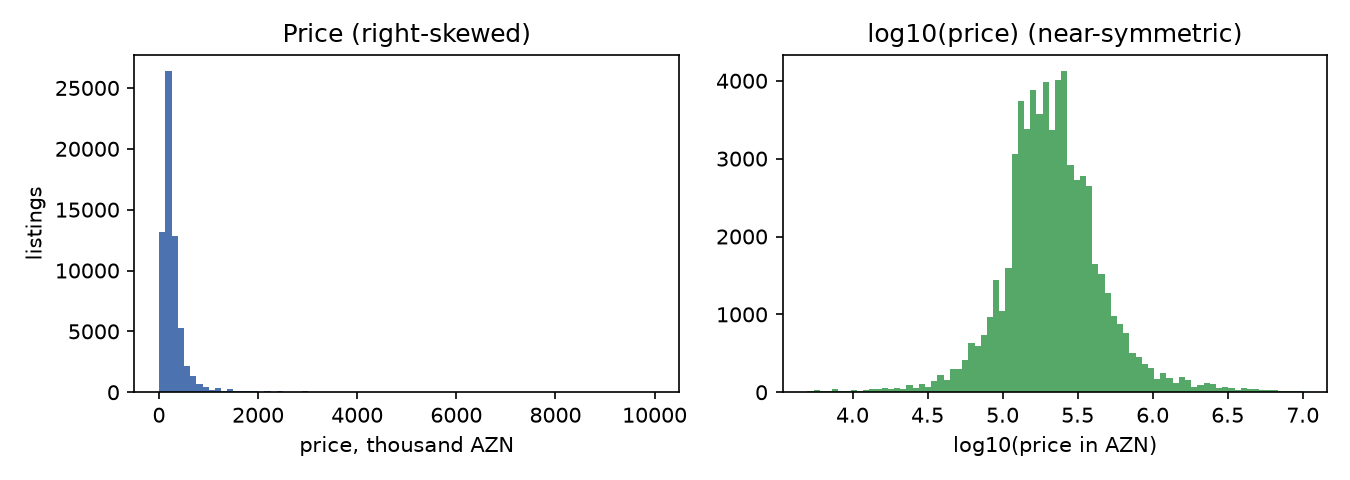
\includegraphics[width=\linewidth]{eda_price_distribution.png}\\[2pt]
  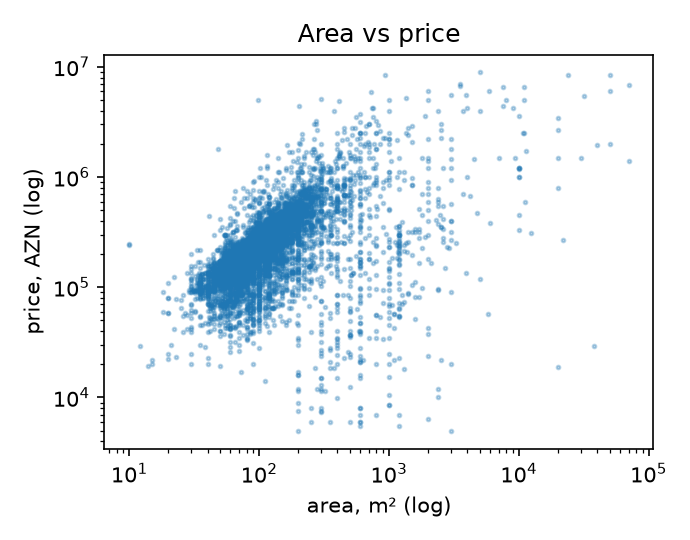
\includegraphics[width=0.49\linewidth]{eda_area_vs_price.png}\hfill
  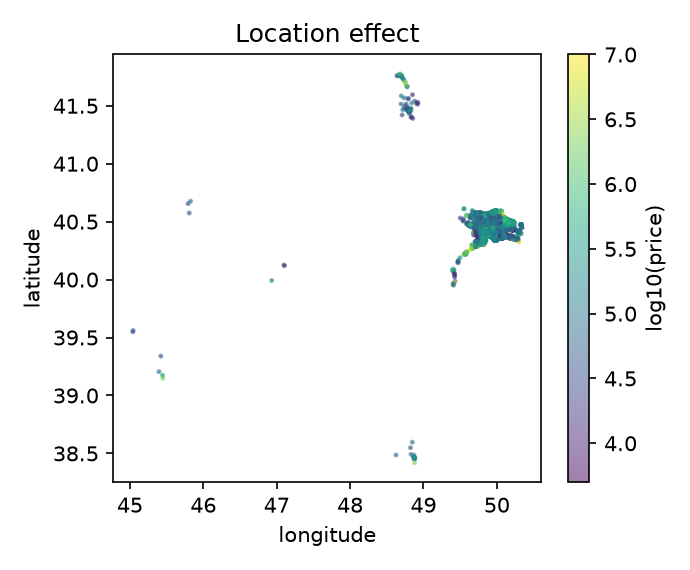
\includegraphics[width=0.49\linewidth]{eda_location.png}
  \caption{EDA. Top: price and $\log_{10}$(price) histograms. Bottom left:
  area vs.\ price (log--log). Bottom right: listing coordinates coloured
  by $\log_{10}$(price); the dense cluster is Baku/Absheron.}
  \label{fig:eda}
\end{figure}

\subsection{Task framing and metrics}
\textbf{Task A} (regression) predicts the price in AZN with the tree
regressor; we report RMSE, MAE and $R^2$, and additionally train a variant
on $\log(\text{price})$ (predictions exponentiated back).
\textbf{Task B} (binary classification) predicts the premium tier with the
tree classifier and both SVMs; we report accuracy, precision, recall, F1,
ROC-AUC, PR-AUC and the confusion matrix. Because the tier is balanced by
construction, accuracy and F1 are meaningful, and the AUCs measure ranking
quality independently of the threshold.

% =====================================================================
\section{Method}
\subsection{Decision tree (from scratch)}
\texttt{DecisionTree} (\texttt{src/decision\_tree.py}) follows the
scikit-learn \texttt{fit}/\texttt{predict}/\texttt{predict\_proba} API and
supports \texttt{task}$\in$\{classification, regression\} with
\texttt{criterion}$\in$\{gini, entropy\} or \{mse\}.

\emph{Split search.} For every feature the node's rows are sorted once;
cumulative class counts (classification) or cumulative sums of $y$ and
$y^2$ (regression, on centred $y$ to avoid float cancellation with large
prices) give the impurity of \emph{every} left/right partition in one
vectorised pass. Cuts are only allowed between two distinct values and
must leave \texttt{min\_samples\_leaf} rows on each side. The threshold is
the midpoint of the two neighbouring values, as in scikit-learn; on ties the
first feature wins.

\emph{Growth and stopping.} The tree is built recursively. A node becomes a
leaf if it reaches \texttt{max\_depth}, has fewer than
\texttt{min\_samples\_split} rows, is pure, has no valid split, or if the
weighted decrease $\frac{N_t}{N}\Delta I$ is below
\texttt{min\_impurity\_decrease} (same scale as scikit-learn). A unit test
checks that each of the four hyperparameters changes the fitted tree.

\emph{Leaves and importances.} Leaves store class frequencies (prediction
by majority, \texttt{predict\_proba} from the frequencies) or the mean
target. Feature importance is the normalised sum of weighted impurity
decreases of the splits that use the feature.

\emph{Tests.} The test suite checks that our tree reproduces scikit-learn's
splits on tiny, fully determined examples for both tasks, matches it exactly
on random regression data, has the same root gain for Gini and entropy, and
that the chosen split is optimal by brute force.

\subsection{Support-vector machine (from scratch)}
\texttt{PegasosSVM} (\texttt{src/svm.py}) minimises~\eqref{eq:primal}
with labels mapped to $\{-1,+1\}$. The bias is folded into $\mathbf x$ as a
constant feature. Each step samples a mini-batch $B$ of $k=64$ rows and
applies
\begin{equation}
  \mathbf w \leftarrow (1-\eta_t\lambda)\,\mathbf w
  + \frac{\eta_t}{k}\sum_{i\in B:\,y_i\mathbf w^\top\mathbf x_i<1} y_i\mathbf x_i ,
\end{equation}
followed by the Pegasos projection onto
$\lVert\mathbf w\rVert\le 1/\sqrt\lambda$. The returned model averages the
iterates of the second half of training, which removes most of the SGD
noise. Exposed hyperparameters are $\lambda$, the training length
(\texttt{n\_iters} or \texttt{n\_epochs}) and the learning-rate schedule:
$\eta_t=1/(\lambda t)$ (Pegasos, default), $\eta_0/\sqrt t$, or constant
$\eta_0$. Features are standardised with training statistics first, since
the hinge loss is scale-sensitive. After fitting, the model reports
$\lVert\mathbf w\rVert$, the margin $2/\lVert\mathbf w\rVert$ and the
support vectors $\{i: y_i(\mathbf w^\top\mathbf x_i+b)\le 1\}$, and keeps
the objective history.

\emph{Non-linearity: random Fourier features.} \texttt{RBFPegasosSVM} maps
$\mathbf x\mapsto\sqrt{2/D}\cos(W^\top\mathbf x+\mathbf c)$ with
$W_{jl}\sim\mathcal N(0,2\gamma)$, $c_l\sim U[0,2\pi]$ and $D=300$, so that
inner products approximate the RBF kernel $e^{-\gamma\lVert\mathbf
x-\mathbf x'\rVert^2}$, and runs the same linear solver. We chose RFF over
kernelised Pegasos because the kernel version needs kernel evaluations
against all $\sim$45k training rows per step and at prediction time,
whereas RFF keeps training linear in $n$. A test checks that the RFF inner
products approximate the exact kernel.

% =====================================================================
\section{Experimental Setup}
\textbf{Protocol.} All randomness is seeded (\texttt{SEED=42}); one command,
\texttt{python -m src.run\_all}, reproduces every number and figure in
about 7 minutes. Hyperparameters are selected on the validation split only.
The test split is used once, for the final numbers.

\textbf{Grids.} Task A tree: \texttt{max\_depth}$\in\{2,4,\dots,14,18\}$,
then \texttt{min\_samples\_leaf}$\in\{1,5,20,50\}$ (selected by
validation RMSE). Task B tree: Gini vs.\ entropy $\times$ the same depths,
then \texttt{min\_samples\_leaf} (selected by validation F1). Linear SVM:
$\lambda\in\{10^{-6},\dots,10^{-1}\}$, 20{,}000 steps of batch 64
($\approx$28 epochs). RBF SVM: $\lambda\in\{10^{-5},10^{-4},10^{-3}\}$
$\times$ $\gamma\in\{0.25/d,\,1/d\}$ with $d=91$. We also study training
length (0.1--30 epochs) and the three learning-rate schedules.

\textbf{Baselines (matched settings).} For the trees we use
\texttt{DecisionTree\-Regressor} and \texttt{DecisionTree\-Classifier} with the same criterion, depth and leaf
size. \texttt{SGDClassifier(loss="hinge", alpha=}$\lambda$\texttt{)} and
\texttt{SVC(kernel="rbf", gamma=}$\gamma$, $C=1/(\lambda n)$\texttt{)},
both inside a \texttt{Pipeline} with \texttt{StandardScaler}. \texttt{SVC}
is trained on a seeded 8{,}000-row subsample because its quadratic cost
makes the full training set impractical.

\textbf{Uncertainty.} Test metrics carry the standard deviation over 200
bootstrap resamples of the test set. In addition we run 5-fold
cross-validation on train+val with the selected hyperparameters; inside each
fold the imputation medians, scaler and tier threshold are re-learned on
the fold's training part.

% =====================================================================
\section{Results}
\subsection{Tuning: bias--variance behaviour}
For Task A, training $R^2$ rises monotonically with depth (0.33 at depth 2
to 0.99 at depth 18) while validation $R^2$ peaks at depth 8 (0.511) and
falls to 0.43 at depth 14--18: the classic overfitting curve
(Fig.~\ref{fig:tuning}, left). Larger leaves regularise further: with
depth 8, \texttt{min\_samples\_leaf}$=50$ lifts validation $R^2$ to 0.579
(RMSE 312k), which is our final regressor. For Task B, Gini and entropy
behave almost identically (Fig.~\ref{fig:tuning}, right); the best
validation F1 is Gini at depth 14 (0.919 vs.\ 0.913 for entropy at the same
depth), and here \texttt{min\_samples\_leaf}$=1$ was best. The train--validation
gap (0.968 vs.\ 0.919) shows that this tree is in the high-variance regime,
but validation F1 has plateaued rather than collapsed.

\begin{figure}[t]
  \centering
  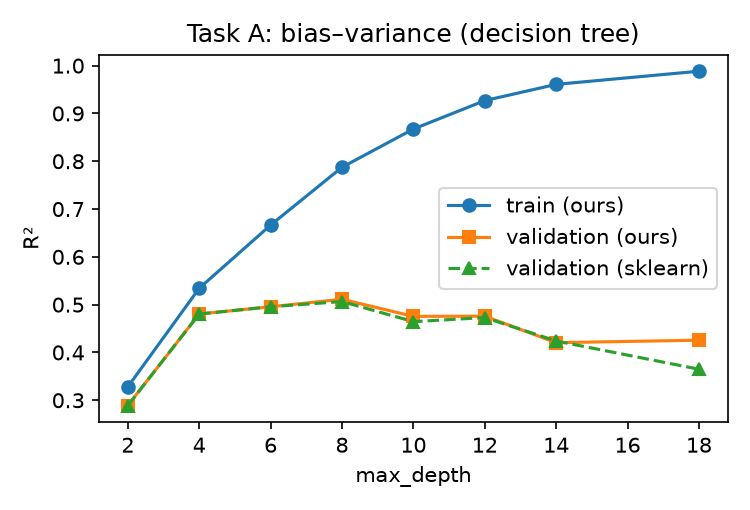
\includegraphics[width=0.49\linewidth]{task_a_depth_curve.png}\hfill
  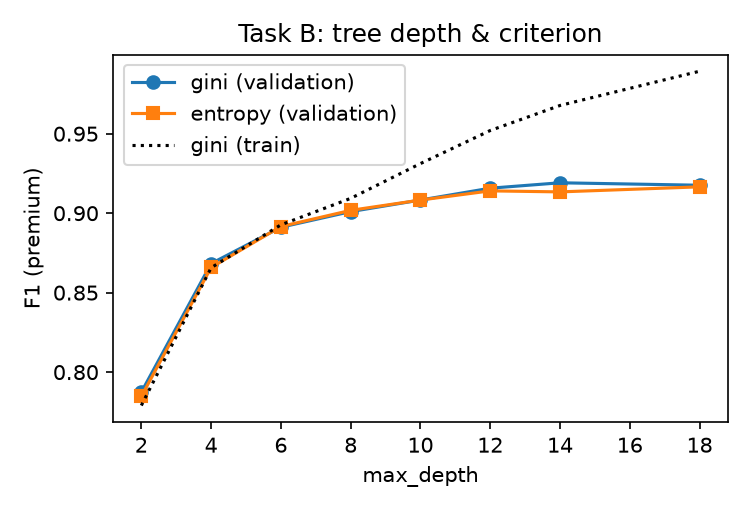
\includegraphics[width=0.49\linewidth]{task_b_tree_depth_criterion.png}
  \caption{Validation curves of our tree. Left: Task A $R^2$ vs.\ depth
  (ours and scikit-learn overlap). Right: Task B F1 vs.\ depth for Gini and
  entropy.}
  \label{fig:tuning}
\end{figure}

For the linear SVM, $\lambda$ trades margin against fit
(Fig.~\ref{fig:svm}): from $\lambda=10^{-6}$ to $10^{-1}$ the margin widens
from 0.013 to 1.82 and the number of support vectors grows from 7{,}073 to
24{,}315, while validation F1 is flat ($\approx$0.844) up to $10^{-2}$ and
drops to 0.825 at $10^{-1}$. We select $\lambda=10^{-3}$ (val F1 0.845):
$\lVert\mathbf w\rVert=2.57$, margin $2/\lVert\mathbf w\rVert=0.78$, and
16{,}906 support vectors (38\% of the training set, as expected for two
heavily overlapping classes). The primal objective decreases for every
$\lambda$; small $\lambda$ converges slowly because the step size
$1/(\lambda t)$ is large. With $\lambda=10^{-3}$, $J$ falls from 2.66
after 0.1 epochs to 0.39 after 30 epochs, while the margin grows from
0.08 to 0.78; the three learning-rate schedules converge to the same
objective ($J\approx0.38$--$0.39$, val F1 0.844--0.845). A 2-D model on
standardised log-area and rooms visualises the effect of $\lambda$: the
margin widens from 1.13 to 2.15 and the boundary rotates when $\lambda$
goes from $10^{-4}$ to $10^{-1}$. For the RBF model the smaller bandwidth
$\gamma=0.25/d$ and $\lambda=10^{-5}$ are best (val F1 0.847, ROC-AUC 0.931);
$\gamma=1/d$ and larger $\lambda$ are consistently worse.

\begin{figure}[t]
  \centering
  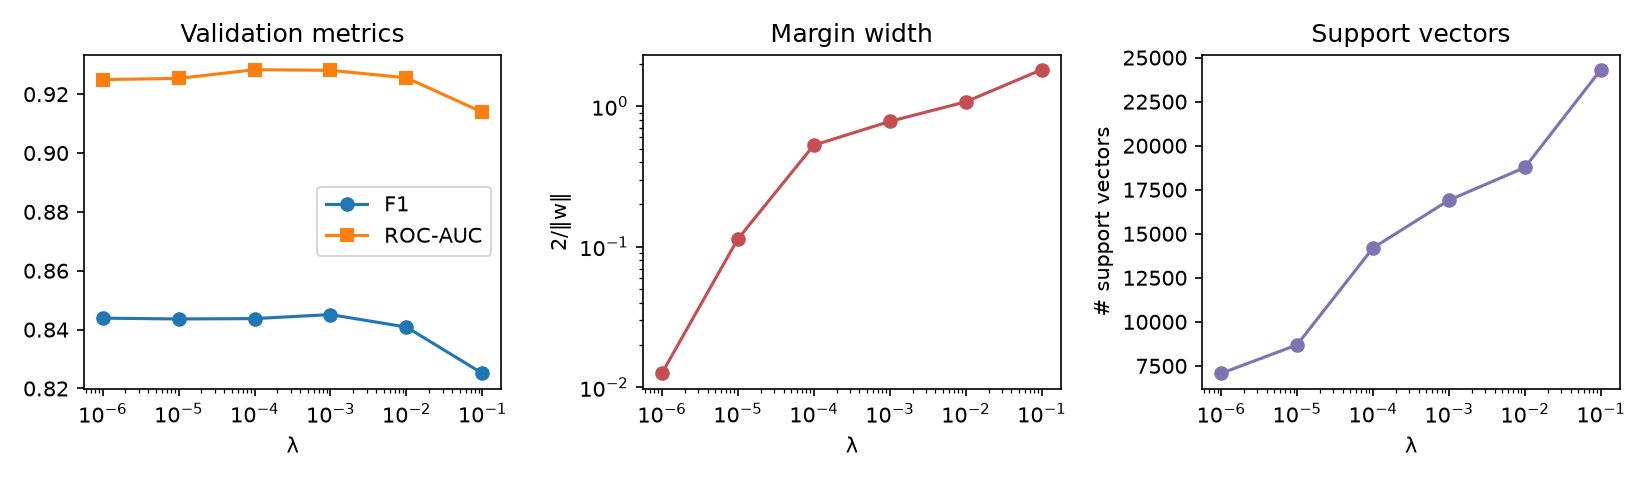
\includegraphics[width=\linewidth]{svm_lambda_sweep.png}\\[2pt]
  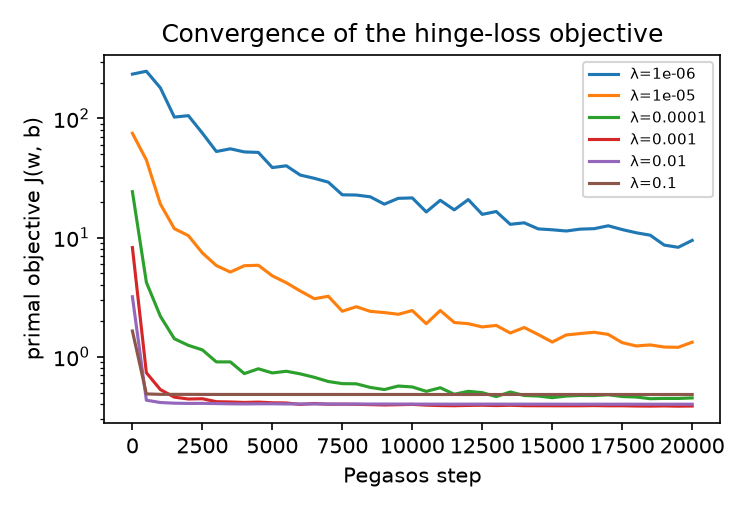
\includegraphics[width=0.49\linewidth]{svm_convergence.png}\hfill
  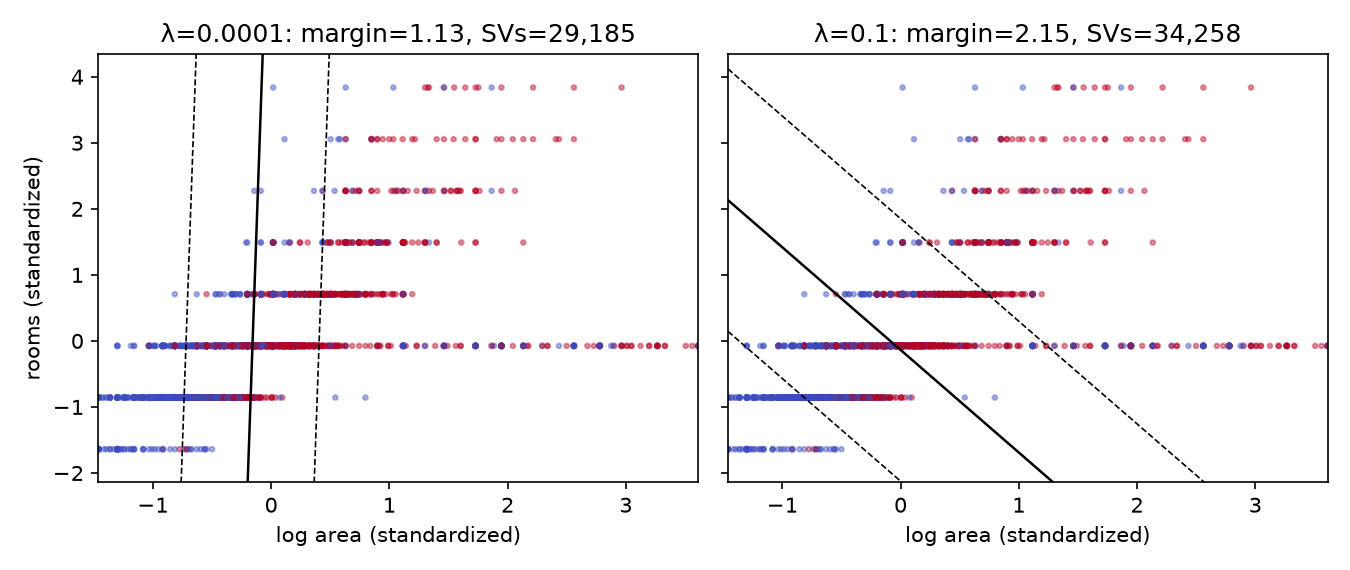
\includegraphics[width=0.49\linewidth]{svm_decision_boundary.png}
  \caption{Pegasos SVM. Top: validation F1/AUC, margin $2/\lVert\mathbf w\rVert$
  and support-vector count vs.\ $\lambda$. Bottom left: primal objective
  vs.\ step. Bottom right: 2-feature boundary and margins for
  $\lambda=10^{-4}$ and $10^{-1}$.}
  \label{fig:svm}
\end{figure}

\subsection{Benchmark against scikit-learn}
Table~\ref{tab:results} is the required results table.

\emph{Trees.} With matched settings our regressor and scikit-learn's have
the same depth and the same 119 leaves; their test predictions correlate at
0.99999 and 90.2\% are identical. On Task B both trees reach depth 14 with
1{,}715 vs.\ 1{,}712 leaves and 99.1\% identical test predictions. The
remaining gaps come from tie-breaking: when two features (or two thresholds)
give exactly the same gain, we keep the first one while scikit-learn visits
features in a random permutation, so a different but equally good split is
taken and the sub-trees diverge below it. Midpoint thresholds between
floating-point values can also differ in the last bit. All differences are
far inside the bootstrap uncertainty.

\emph{SVMs.} Our linear Pegasos and \texttt{SGDClassifier} with the same
hinge loss and $\lambda$ agree to the third decimal in every metric (test
F1 0.850 vs.\ 0.850, ROC-AUC 0.931 vs.\ 0.930). The RFF model is on a par
with the linear SVM in F1 and slightly better in AUC (0.932, PR-AUC 0.927),
and is about 0.004--0.006 below exact-kernel \texttt{SVC} on every metric.
The gap is small given that SVC sees the exact kernel while RFF uses a
300-dimensional approximation, but SVC also sees only 8{,}000 rows.

\emph{Cross-validation} (Table~\ref{tab:results}, bottom) confirms the
ranking: our trees and our linear SVM are within one fold standard
deviation of their scikit-learn counterparts on every metric, and the RFF
model again sits slightly below \texttt{SVC} (ROC-AUC 0.928 vs.\ 0.932). Task A test RMSE (342k) is higher than the CV
mean (310k) because a few very expensive listings in the test split
dominate the squared error, which the large bootstrap std ($\pm$19k) also
shows.

\emph{Speed.} Our pure-Python tree is slower to fit (1.7~s vs.\ 0.3~s on
Task A, 10.4~s vs.\ 0.6~s for the deep Task B tree) because the recursion
and per-node sorting run in Python rather than Cython, and prediction walks
the tree row by row. Our SVM fits as fast as \texttt{SGDClassifier}
($\approx$1.7~s) and predicts faster (one matrix product). \texttt{SVC}
needed 2.2~s to fit on only 8{,}000 rows and 3.7~s to predict, and its cost
grows roughly quadratically with $n$, whereas Pegasos is linear in $n$.

\begin{table*}[t]
  \centering
  \caption{Results on both tasks. Top: held-out test set (mean $\pm$ bootstrap
  std over 200 resamples). Bottom: 5-fold cross-validation on train+val
  (mean $\pm$ std over folds). Times in seconds on the full training set.
  Best value per column in bold.}
  \label{tab:results}
  \footnotesize
  \setlength{\tabcolsep}{3pt}
  \resizebox{\textwidth}{!}{%
  \begin{tabular}{@{}l ccc c cccc cc@{}}
    \toprule
    & \multicolumn{3}{c}{Task A: regression (AZN)} && \multicolumn{4}{c}{Task B: price tier} & \multicolumn{2}{c}{Time (s)}\\
    \cmidrule{2-4}\cmidrule{6-9}\cmidrule{10-11}
    Model & RMSE & MAE & $R^2$ && Accuracy & F1 & ROC-AUC & PR-AUC & fit & predict \\
    \midrule
    \multicolumn{11}{@{}l}{\emph{Test set}}\\
    Ours: tree (MSE / Gini)             & 342{,}525 $\pm$ 19{,}432 & 102{,}958 $\pm$ 2{,}944 & 0.533 $\pm$ 0.031 && \textbf{0.922} $\pm$ .003 & \textbf{0.922} $\pm$ .003 & 0.924 $\pm$ .003 & 0.882 $\pm$ .006 & 1.7 / 10.4 & 0.03 / 0.05\\
    sklearn: DecisionTree               & \textbf{342{,}515} $\pm$ 19{,}432 & 102{,}938 $\pm$ 2{,}943 & \textbf{0.533} $\pm$ 0.031 && 0.920 $\pm$ .003 & 0.919 $\pm$ .003 & 0.920 $\pm$ .003 & 0.874 $\pm$ .006 & 0.3 / 0.6 & 0.003 / 0.004\\
    Ours: tree, log-price target        & 365{,}036 $\pm$ 24{,}456 & \textbf{98{,}963} $\pm$ 3{,}283 & 0.470 $\pm$ 0.029 && -- & -- & -- & -- & -- & 0.02\\
    Ours: SVM (Pegasos, linear)         & n/a & n/a & n/a && 0.850 $\pm$ .004 & 0.850 $\pm$ .004 & 0.931 $\pm$ .002 & 0.922 $\pm$ .004 & 1.7 & 0.001\\
    sklearn: SGD hinge [Pipeline]       & n/a & n/a & n/a && 0.850 $\pm$ .004 & 0.850 $\pm$ .004 & 0.930 $\pm$ .002 & 0.920 $\pm$ .004 & 1.8 & 0.005\\
    Ours: SVM (Pegasos + RFF, RBF)      & n/a & n/a & n/a && 0.849 $\pm$ .004 & 0.849 $\pm$ .004 & 0.932 $\pm$ .002 & 0.927 $\pm$ .003 & 1.9 & 0.07\\
    sklearn: SVC RBF [Pipeline, 8k rows]& n/a & n/a & n/a && 0.854 $\pm$ .004 & 0.855 $\pm$ .004 & \textbf{0.936} $\pm$ .002 & \textbf{0.931} $\pm$ .003 & 2.2 & 3.7\\
    \midrule
    \multicolumn{11}{@{}l}{\emph{5-fold cross-validation}}\\
    Ours: tree                          & 310{,}469 $\pm$ 18{,}477 & 98{,}608 $\pm$ 3{,}711 & 0.588 $\pm$ 0.024 && 0.918 $\pm$ .003 & 0.917 $\pm$ .003 & 0.924 $\pm$ .004 & 0.894 $\pm$ .009 & & \\
    sklearn: DecisionTree               & 310{,}493 $\pm$ 18{,}520 & 98{,}619 $\pm$ 3{,}730 & 0.588 $\pm$ 0.024 && 0.918 $\pm$ .003 & 0.917 $\pm$ .004 & 0.924 $\pm$ .004 & 0.893 $\pm$ .010 & & \\
    Ours: SVM (linear)                  & n/a & n/a & n/a && 0.847 $\pm$ .005 & 0.846 $\pm$ .006 & 0.927 $\pm$ .003 & 0.913 $\pm$ .007 & & \\
    sklearn: SGD hinge [Pipeline]       & n/a & n/a & n/a && 0.845 $\pm$ .004 & 0.843 $\pm$ .005 & 0.926 $\pm$ .003 & 0.912 $\pm$ .006 & & \\
    Ours: SVM (RBF, RFF)                & n/a & n/a & n/a && 0.845 $\pm$ .005 & 0.845 $\pm$ .006 & 0.928 $\pm$ .003 & 0.922 $\pm$ .004 & & \\
    sklearn: SVC RBF [subsample]        & n/a & n/a & n/a && 0.850 $\pm$ .004 & 0.848 $\pm$ .005 & 0.932 $\pm$ .003 & 0.926 $\pm$ .005 & & \\
    \bottomrule
  \end{tabular}}
  \\[3pt]
  \footnotesize Tree times are Task A / Task B. Precision and recall (all models
  0.84--0.92, balanced within 0.01--0.02) are listed in \texttt{report/results.txt}.
\end{table*}

\subsection{Tree vs.\ SVM on Task B}
The tree has the best F1 (0.922 vs.\ 0.850) but the lowest ROC-AUC (0.924
vs.\ 0.931--0.936). The confusion matrices (Fig.~\ref{fig:clf}) show where
the F1 gap comes from: the tree makes 747 errors on 9{,}637 test listings,
the linear SVM 1{,}444, with errors split evenly between false premium and
false standard for both. The tree can carve out location- and
category-specific regions that a single hyperplane over 91 features cannot.
Its AUC is lower because a depth-14 tree has many almost pure leaves, so
its scores take few distinct values and give a coarse ranking; the ROC curve
of the tree is a few long straight segments. Interestingly, the depth-8
tree had a higher validation AUC (0.958) than the depth-14 tree (0.927):
we selected on F1 as planned, and a practitioner who needs a ranking
should choose the shallower tree.

\begin{figure}[t]
  \centering
  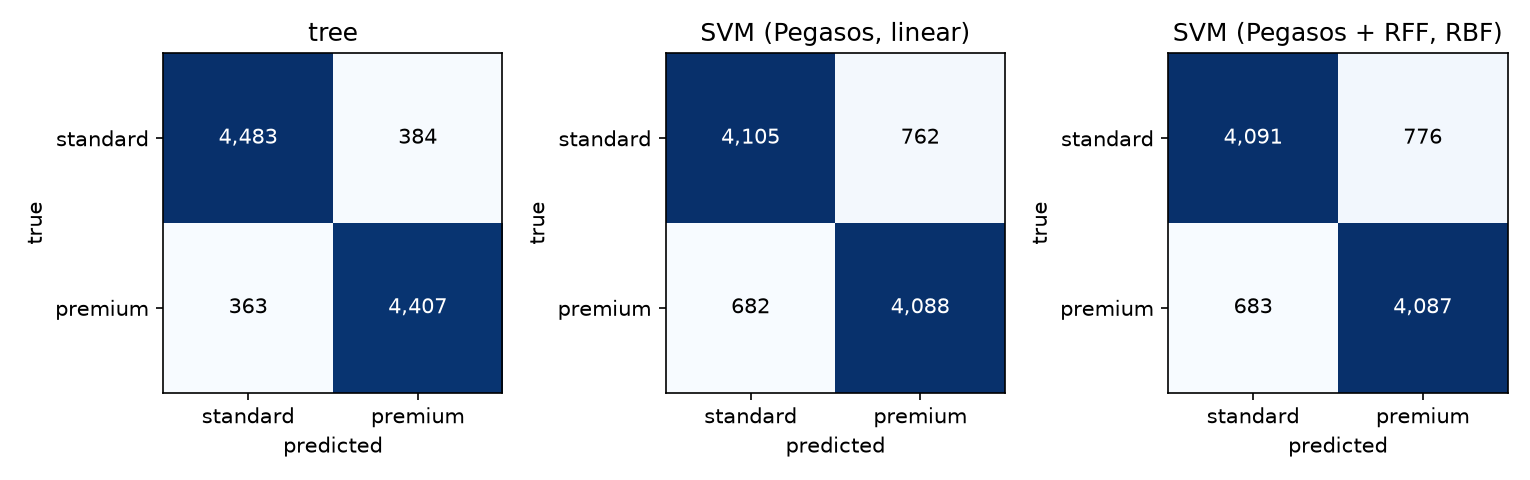
\includegraphics[width=\linewidth]{task_b_confusion_matrices.png}\\[2pt]
  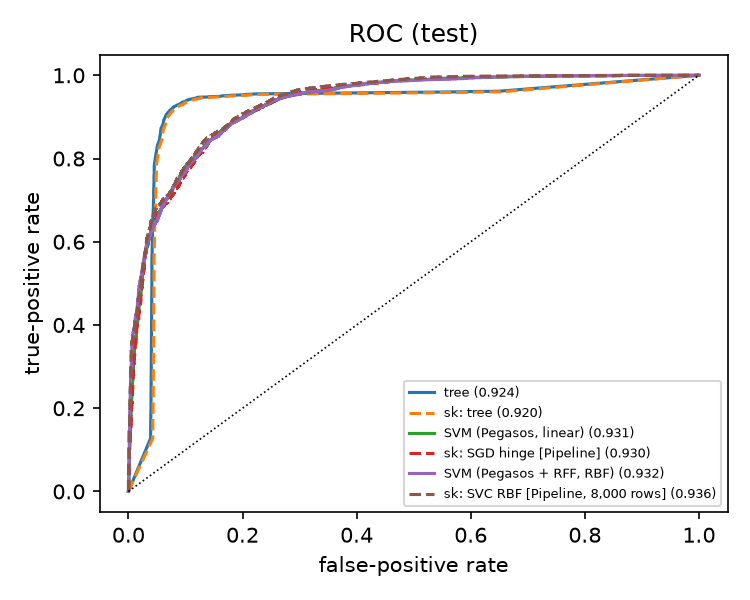
\includegraphics[width=0.62\linewidth]{task_b_roc.png}
  \caption{Task B on the test set: confusion matrices of our three models
  (top) and ROC curves of all six models (bottom, AUC in the legend).}
  \label{fig:clf}
\end{figure}

% =====================================================================
\section{Error Analysis}
\subsection{What the models use}
Tree importances (Fig.~\ref{fig:imp}) are dominated by area (0.59 in
Task A, 0.51 in Task B). In Task A the second feature is the
\emph{Obyekt} (commercial) category (0.22), which separates the most
expensive segment, followed by latitude, land plots (\emph{Torpaq}) and
longitude. In Task B, where the question is ``above or below 210k'',
location becomes more important: longitude (0.18) and latitude (0.13) are
the next features after area, followed by land area and floor.

The SVM weights on standardised features tell a consistent story: rooms
($+1.65$) and area ($+1.16$) push towards premium, as does the new-build
category ($+0.52$) and central districts such as Şah İsmayıl Xətai and
Ağ şəhər ($+0.32$). Suburban settlements (Masazır, Hövsan; $-0.43$,
$-0.34$) and houses/country houses ($-0.40$) push towards standard. Rooms
outweighs area in the SVM, unlike in the tree, because the two are strongly
correlated and the linear model splits their shared effect; their sum is
what matters.

\begin{figure}[t]
  \centering
  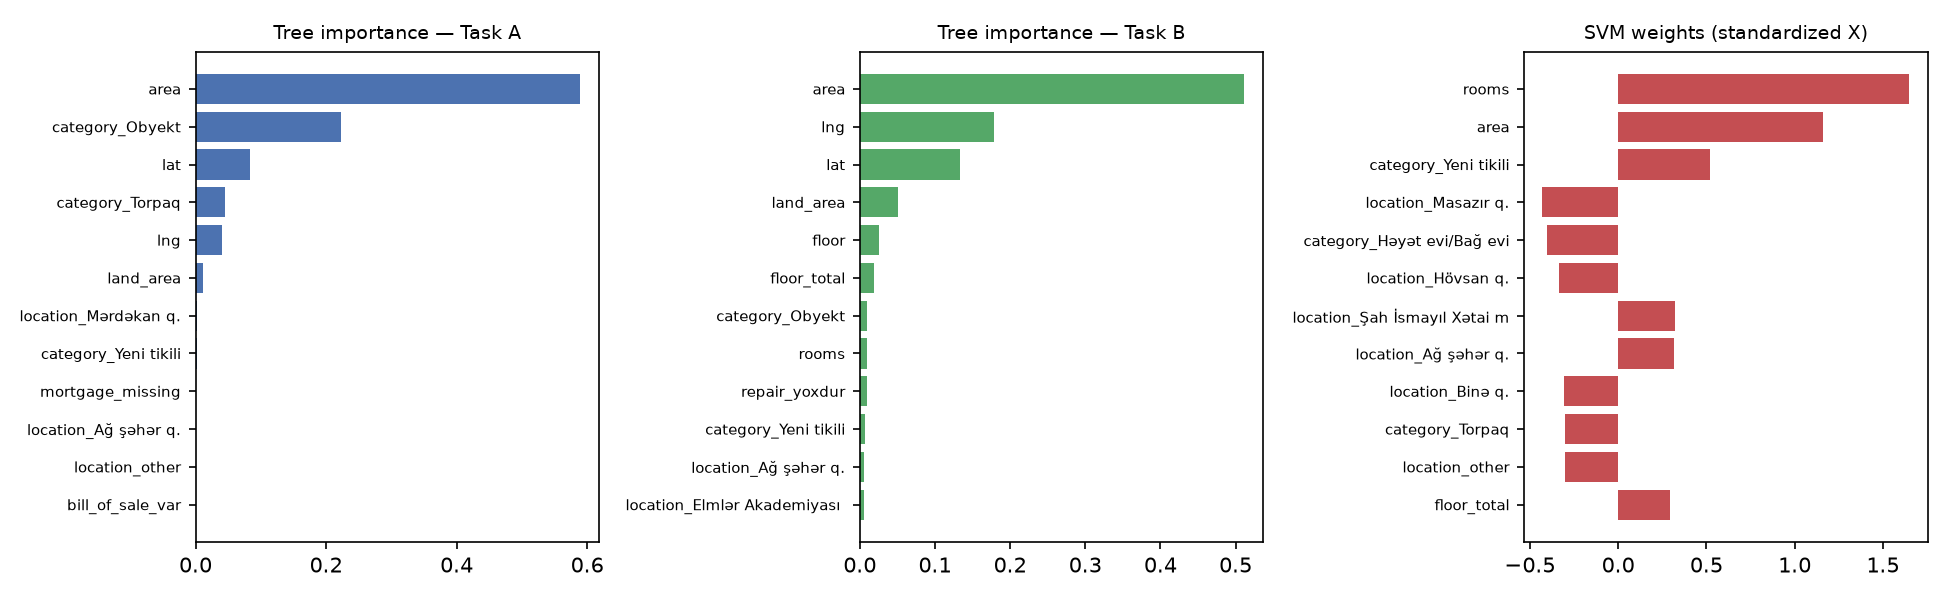
\includegraphics[width=\linewidth]{feature_importance.png}
  \caption{Tree impurity-decrease importances (Task A, Task B) and the 12
  largest linear SVM weights on standardised features.}
  \label{fig:imp}
\end{figure}

\subsection{Where the models fail}
\textbf{Property type.} Regression error is low for flats (median absolute
percentage error, MdAPE, 14.2\% for new builds and 15.3\% for old stock,
which make up 76\% of the test set) and much higher for houses (27.4\%),
commercial objects (46.9\%) and land plots (60.8\%;
Fig.~\ref{fig:errors}). Land and commercial prices depend on things the data
does not describe well (zoning, frontage, the business inside), and these
segments have few examples.

\textbf{Luxury and cheap listings.} By test price quartile, MdAPE is
23.5\% (Q1), 13.5\% (Q2), 14.8\% (Q3) and 21.3\% (Q4); the tree regresses
towards the middle of the market. In absolute terms the luxury quartile
dominates: its MAE is 268k~AZN against 37--58k for Q1--Q3, which is why
RMSE is so much larger than MAE. The log-price model reduces the MAE
(99.0k vs.\ 103.0k) by fitting relative errors better, but increases RMSE
because it under-predicts the most expensive listings.

\textbf{Sparse districts.} Listings whose district had fewer than 100
training examples (merged into \texttt{location\_other}, 4.6\% of the test
set) have an MdAPE of 49.6\% vs.\ 16.7\% elsewhere, and a tier error of
11.8\% vs.\ 7.6\%. The model has no district information for them and has
to rely on coordinates, which are themselves sparse outside Baku.

\textbf{Near the tier threshold.} For the Task B tree, 24.3\% of listings
priced within $\pm$15\% of 210k~AZN are misclassified, against 4.0\%
elsewhere. Many of these errors are unavoidable: two similar flats can be
listed at 200k and 220k.

\begin{figure}[t]
  \centering
  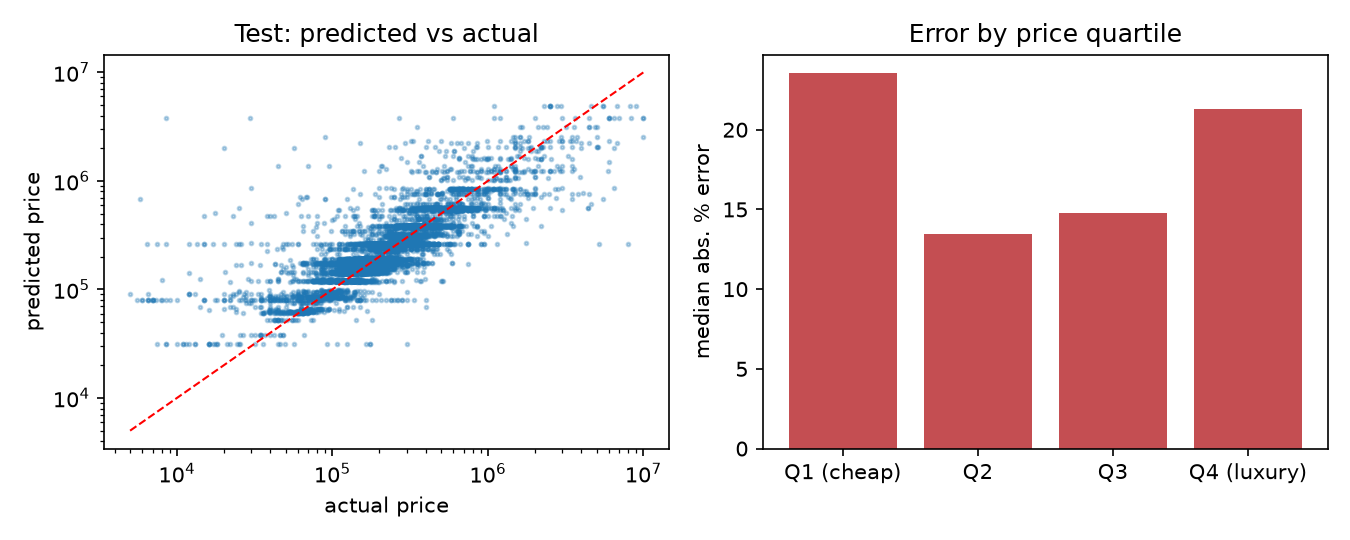
\includegraphics[width=\linewidth]{task_a_errors.png}\\[2pt]
  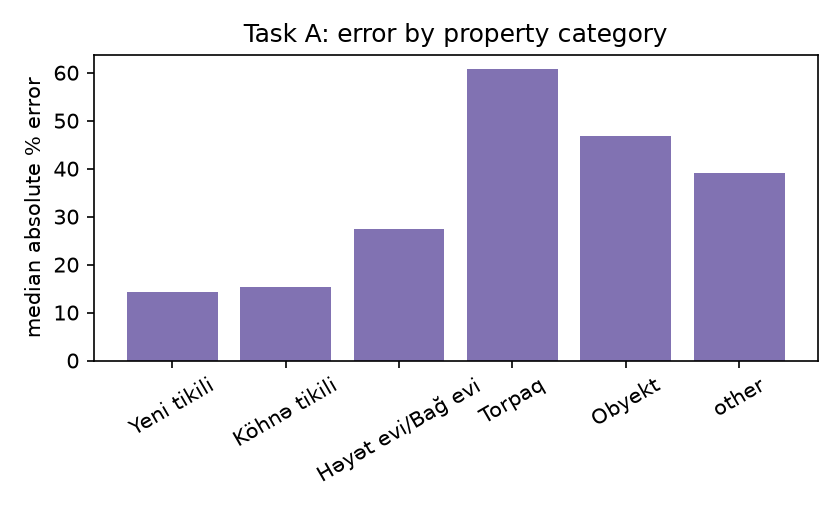
\includegraphics[width=0.62\linewidth]{task_a_error_by_category.png}
  \caption{Task A errors of our tree on the test set: predicted vs.\ actual
  price and MdAPE by price quartile (top); MdAPE by property category
  (bottom).}
  \label{fig:errors}
\end{figure}

% =====================================================================
\section{Discussion and Limitations}
\begin{itemize}
  \setlength\itemsep{0pt}
  \item \emph{Moderate regression quality.} A single depth-8 tree explains
        about 53--59\% of the price variance. The piecewise-constant
        prediction is visible as horizontal bands in Fig.~\ref{fig:errors};
        ensembles (the optional bonus, not done) would smooth this.
  \item \emph{Raw-price metric.} Task A is evaluated on raw AZN, so RMSE is
        dominated by a few expensive listings; MdAPE and the log-price
        variant give a complementary view.
  \item \emph{Balanced tier by construction.} The median split makes the
        classes balanced and the threshold arbitrary; listings near it are
        inherently hard.
  \item \emph{SVC on a subsample.} The exact-kernel baseline uses 8{,}000
        rows, so the RFF--SVC comparison mixes two effects (kernel
        approximation vs.\ less data).
  \item \emph{Unused information.} Free-text descriptions and listing
        attributes were dropped; they likely contain renovation quality,
        view and building details that would help most for houses and
        commercial objects.
  \item \emph{Data snapshot.} One scrape of one platform; asking prices are
        not transaction prices, and fixed outlier bounds may still keep some
        mistyped prices.
  \item \emph{Speed.} Our tree is 5--18$\times$ slower to fit than
        scikit-learn's Cython implementation.
\end{itemize}

\section{Conclusion}
A carefully cleaned, leakage-free version of the bina.az dump supports
both tasks well. Our NumPy decision tree reproduces scikit-learn's trees
almost split for split, and our Pegasos SVM matches the hinge-loss
\texttt{SGDClassifier} to three decimals; RFF brings it within 0.005 AUC of
an exact RBF \texttt{SVC} at a fraction of the cost. For the price tier,
the tree is the more accurate classifier and the SVM the better ranker.
Most of the remaining error sits in land plots, commercial objects, luxury
listings and rarely listed districts. Next steps are a random forest or
gradient boosting built from our own trees, text features from the listing
descriptions, and geographic clustering of the coordinates to replace the
sparse district levels.

\section*{Team Contributions}
% Fill in from contribution_report.md
{\raggedright\noindent\textbf{All members:} data cleaning and EDA
(\texttt{src/data\_prep.py}, tests).\\
\textbf{Araz Valishov, Elsaf Baghirov:} decision tree (\texttt{src/decision\_tree.py},
tests), tree experiments.\\
\textbf{Huseynali Mehdiyev, Joshgun Malikov:} Pegasos SVM and RFF (\texttt{src/svm.py},
tests), SVM experiments.\\
\textbf{Huseynali Mehdiyev, Araz Valishov:} benchmark and error analysis (\texttt{src/run\_all.py},
\texttt{src/evaluate.py}), report and slides. Details in
\texttt{contribution\_report.md}.\par}

\section*{Tools and Acknowledgements}
Data: bina.az sale listings, Kaggle dataset
\texttt{sehriyarmemmedli/binaaz-sale-project}. Software: NumPy, pandas,
Matplotlib; scikit-learn only for the baselines and the sanity tests.
AI-assistance disclosure: an AI assistant (Claude, Anthropic) was used to
help draft the text of this report and the slides from our
results files and figures. All numbers come from \texttt{report/results.txt}
produced by our code, and the team reviewed and edited the text.

% =====================================================================
\begin{thebibliography}{9}
\bibitem{pegasos}
S.~Shalev-Shwartz, Y.~Singer, N.~Srebro, and A.~Cotter,
``Pegasos: primal estimated sub-gradient solver for SVM,''
\emph{Mathematical Programming}, vol.~127, no.~1, pp.~3--30, 2011.
\bibitem{rff}
A.~Rahimi and B.~Recht, ``Random features for large-scale kernel
machines,'' in \emph{Advances in Neural Information Processing Systems
20}, 2007, pp.~1177--1184.
\bibitem{breiman}
L.~Breiman, J.~Friedman, R.~Olshen, and C.~Stone, \emph{Classification
and Regression Trees}. Wadsworth, 1984.
\bibitem{sklearn}
F.~Pedregosa \emph{et al.}, ``Scikit-learn: machine learning in Python,''
\emph{Journal of Machine Learning Research}, vol.~12, pp.~2825--2830, 2011.
\end{thebibliography}

\end{document}
